% presentaciones/sesion01-cap01/sesion01.tex
% Sesión 1 — Capítulo 1: El consumidor digital: evolución, impacto y ventajas de su análisis
% Laboratorio: Gestión de datos, comportamiento y perfiles del consumidor digital
% Lic. en Mercadotecnia Digital · ESCA Unidad Santo Tomás · IPN
% Fuente de contenido: libro-consumidor-digital/partes/parte1/cap01.tex
% Figuras reutilizadas del libro (TikZ y MATLAB) sin copiarlas: ver \graphicspath y \input.
\documentclass[aspectratio=169,xcolor=dvipsnames]{beamer}
\usetheme{Berlin}

%----------------------------------------------------------------------------------------
%   PALETA INSTITUCIONAL IPN (Manual de Identidad Gráfica, Pantone 222C)
%----------------------------------------------------------------------------------------
\usepackage[dvipsnames,svgnames,x11names]{xcolor}
\definecolor{IPNguinda}{HTML}{6F1D46}       % Pantone 222C oficial — color primario
\definecolor{IPNguindaOsc}{HTML}{45102C}    % sombra / paleta secundaria
\definecolor{IPNguindaClara}{HTML}{F4E9EF}  % fondo de bloques normales
\definecolor{IPNdorado}{HTML}{B8975A}       % dorado — SOLO enlaces y detalles del cierre
\definecolor{IPNterracota}{HTML}{9C5B44}    % alertblock
\definecolor{IPNterracotaClara}{HTML}{F6ECE6}
\definecolor{IPNbronce}{HTML}{8C6B3F}       % exampleblock
\definecolor{IPNbronceClaro}{HTML}{F5F0E3}
\definecolor{IPNgris}{HTML}{58595B}         % texto secundario / notas

% Alias con los nombres de config/colores.tex del libro, para que las figuras
% TikZ del libro se puedan \input sin modificarlas
\colorlet{guindaIPN}{IPNguinda}
\colorlet{guindaIPNOsc}{IPNguindaOsc}
\colorlet{guindaIPNClara}{IPNguindaClara}
\colorlet{doradoIPN}{IPNdorado}
\colorlet{bronceIPN}{IPNbronce}
\colorlet{bronceIPNClaro}{IPNbronceClaro}
\colorlet{grisIPN}{IPNgris}
\definecolor{colorLaboratorio}{HTML}{1B6E7A}

\setbeamercolor{palette primary}{bg=IPNguinda,fg=white}
\setbeamercolor{palette secondary}{bg=IPNguindaOsc,fg=white}
\setbeamercolor{palette tertiary}{bg=IPNguindaOsc,fg=white}
\setbeamercolor{palette quaternary}{bg=IPNguinda,fg=white}
\setbeamercolor{structure}{fg=IPNguinda}
\setbeamercolor{title}{bg=IPNguinda,fg=white}
\setbeamercolor{frametitle}{bg=IPNguinda,fg=white}
\setbeamercolor{block title}{bg=IPNguinda,fg=white}
\setbeamercolor{block body}{bg=IPNguindaClara,fg=black}
\setbeamercolor{block title alerted}{bg=IPNterracota,fg=white}
\setbeamercolor{block body alerted}{bg=IPNterracotaClara,fg=black}
\setbeamercolor{block title example}{bg=IPNbronce,fg=white}
\setbeamercolor{block body example}{bg=IPNbronceClaro,fg=black}
\setbeamercolor{alerted text}{fg=IPNterracota}
\setbeamercolor{item}{fg=IPNguinda}
\setbeamercolor{section in toc}{fg=IPNguinda}
\setbeamercolor{footline}{bg=IPNguindaOsc,fg=white}

\usepackage[spanish,es-noshorthands,es-nodecimaldot]{babel}
\usepackage{csquotes}
\usepackage{hyperref}
\usepackage{graphicx}
\usepackage{booktabs}
\usepackage{array}
\usepackage{amsmath}
\setbeamertemplate{caption}[numbered]
\usepackage{xurl}
\usepackage{adjustbox}
\usepackage{tikz}
\usetikzlibrary{arrows.meta,positioning}
\usepackage{pgfplots}
\pgfplotsset{compat=1.18}

\graphicspath{{Figures/}{../../libro-consumidor-digital/figuras/matlab/}}
\newcommand{\figtikz}[1]{../../libro-consumidor-digital/figuras/tikz/#1}
\newcommand{\fuente}[1]{{\tiny\color{IPNgris}Fuente: #1}}

\hypersetup{
    colorlinks=true,
    linkcolor=IPNdorado,
    filecolor=IPNguinda,
    urlcolor=IPNguinda,
    citecolor=IPNguinda,
    pdftitle={Sesion 1 - El consumidor digital},
    pdfauthor={Dr. Aboud Barsekh-Onji},
}

%----------------------------------------------------------------------------------------
%   CODE LISTINGS — sintaxis ESTÁNDAR del lenguaje
%----------------------------------------------------------------------------------------
\usepackage{listings}
\definecolor{backcolour}{rgb}{0.97,0.97,0.99}
\definecolor{codegreen}{rgb}{0,0.6,0}

\lstdefinestyle{MATLABStyle}{
  language=Matlab,
  basicstyle=\ttfamily\scriptsize,
  keywordstyle=\color{blue}\bfseries,
  commentstyle=\color{codegreen},
  stringstyle=\color{violet},
  breaklines=true,
  numbers=left,
  numbersep=5pt,
  frame=lines,
  backgroundcolor=\color{backcolour}
}
\lstset{style=MATLABStyle}

%----------------------------------------------------------------------------------------
%   TITLE CONFIGURATION
%----------------------------------------------------------------------------------------
\logo{
\includegraphics[height=0.75cm]{ipn-escudo.png}}
\title[Sesión 1 · El consumidor digital]{El consumidor digital: evolución, impacto\\ y ventajas de su análisis}
\subtitle{Sesión 1 · Unidad I — Capítulo 1}
\author{Dr. Aboud Barsekh-Onji}
\institute[IPN]{
    Instituto Politécnico Nacional \\
    \small ESCA Unidad Santo Tomás · Lic. en Mercadotecnia Digital \\
    \footnotesize Laboratorio: Gestión de datos, comportamiento y perfiles del consumidor digital
}
\date{\today}

%----------------------------------------------------------------------------------------
%   AUTO AGENDA AT EACH SECTION
%----------------------------------------------------------------------------------------
\AtBeginSection[]{
  \begin{frame}{Agenda}
    \tableofcontents[currentsection]
  \end{frame}
}

\begin{document}

\begin{frame}
    \titlepage
    \vspace{-4pt}
    \begin{center}
        {\tiny\color{IPNgris} ORCID: \href{https://orcid.org/0009-0004-5440-8092}{0009-0004-5440-8092}}
    \end{center}
\end{frame}

%------------------------------------------------
\section{Encuadre}
%------------------------------------------------

\begin{frame}{Ficha de la sesión}
\begin{columns}[T]
  \column{0.52\textwidth}
  \begin{block}{Unidad I}
    Comportamiento, perfil y gestión de datos del consumidor digital
  \end{block}
  \begin{block}{Temas del programa (1.1)}
    \small
    \begin{itemize}
      \item[1.1.1] Evolución del consumidor 1.0 al 5.0 y tendencias
      \item[1.1.2] Consumo digital inteligente y sostenible
      \item[1.1.3] Ventajas del análisis del consumidor digital
    \end{itemize}
  \end{block}
  \column{0.44\textwidth}
  \begin{block}{Carga horaria}
    \small Teoría 3.0 h · Práctica 2.0 h\\ Aprendizaje autónomo 1.0 h
  \end{block}
  \begin{exampleblock}{Competencia de la unidad}
    \small Identifica el comportamiento del consumidor digital y su evolución a partir de sus tipos de perfil y gestión de datos.
  \end{exampleblock}
\end{columns}
\end{frame}

\begin{frame}{Al terminar la sesión podrás\ldots}
\begin{enumerate}
  \item \textbf{Distinguir} la evolución real del consumidor digital de su periodización comercial en \enquote{versiones}.
  \vspace{6pt}
  \item \textbf{Explicar}, con al menos dos fuentes verificables, qué significa consumo digital \emph{inteligente} y \emph{sostenible} en el contexto mexicano.
  \vspace{6pt}
  \item \textbf{Argumentar}, con datos, al menos tres ventajas concretas de analizar el comportamiento del consumidor digital para una organización.
\end{enumerate}
\vspace{8pt}
\begin{alertblock}{Regla de la unidad}
  Toda cifra lleva fuente, año y fecha de consulta. Sin fuente, no es dato: es opinión.
\end{alertblock}
\end{frame}

\begin{frame}{Arranque: la lectura previa}
\begin{columns}[T]
  \column{0.55\textwidth}
  Saquen sus respuestas a las preguntas de reflexión.
  \vspace{6pt}
  \begin{exampleblock}{Pregunta 1}
    Piensen en su última compra digital. ¿Qué parte de su decisión fue realmente \textbf{independiente} y qué parte estuvo influida por ver que \textbf{otras personas} ya habían comprado o recomendado lo mismo?
  \end{exampleblock}
  \column{0.41\textwidth}
  \begin{block}{Dinámica (10 min)}
    \small
    \begin{enumerate}
      \item Parejas: comparen respuestas (3 min).
      \item Pizarrón: dos columnas \emph{independiente} / \emph{por imitación}.
      \item Guardamos el pizarrón: vuelve en el laboratorio como $p$ y $q$.
    \end{enumerate}
  \end{block}
\end{columns}
\end{frame}

%------------------------------------------------
\section[Apertura]{Caso de apertura}
%------------------------------------------------

\begin{frame}{Una curva, no una revolución instantánea}
\small
\begin{columns}[c]
  \column{0.52\textwidth}
  \begin{tikzpicture}
    \begin{axis}[
        width=\linewidth, height=4.8cm,
        ybar, bar width=18pt, ymin=0, ymax=100,
        symbolic x coords={2015,2024,2025},
        xtick=data,
        ylabel={\% de la población de 6+ años},
        ylabel style={font=\scriptsize}, tick label style={font=\scriptsize},
        nodes near coords, nodes near coords style={font=\scriptsize},
        enlarge x limits=0.3,
        axis lines*=left, ymajorgrids, grid style={IPNgris!25},
      ]
      \addplot[fill=IPNguinda, draw=IPNguindaOsc] coordinates {(2015,57.4) (2024,83.1) (2025,86.1)};
    \end{axis}
  \end{tikzpicture}\\
  \fuente{INEGI, ENDUTIH 2024 y 2025 (comunicados 57/25 y 32/26).}
  \column{0.44\textwidth}
  \begin{itemize}
    \item Usuarios de internet en México: \textbf{57.4\,\%} (2015) $\rightarrow$ \textbf{86.1\,\%} (2025).
    \item Comercio electrónico 2025: \textbf{\$941 mil millones} de pesos y \textbf{77.2 millones} de compradores digitales \fuente{AMVO, 2026}.
    \item Brecha 2024: urbano \textbf{86.9\,\%} vs.\ rural \textbf{68.5\,\%}.
  \end{itemize}
  \vspace{2pt}
  {\footnotesize Lenta al principio, acelerada después; cerca de su techo en unos segmentos y lejos en otros.}
\end{columns}
\end{frame}

\begin{frame}{La pregunta que abre el capítulo}
\begin{center}
\begin{minipage}{0.85\textwidth}
\begin{block}{}
  \centering\large
  ¿La evolución del consumidor digital es un fenómeno que se \textbf{mide} con esa curva\ldots\\[6pt]
  \ldots o es, además, una \textbf{narrativa} que ciertas editoriales de consultoría han sabido vender en entregas sucesivas?
\end{block}
\end{minipage}
\end{center}
\vspace{10pt}
\pause
\begin{center}
  \textcolor{IPNguinda}{\textbf{Las dos cosas son ciertas.}} Distinguirlas es el primer ejercicio de rigor analítico del curso.
\end{center}
\end{frame}

%------------------------------------------------
\section[Evolución]{1.1.1 Evolución del consumidor}
%------------------------------------------------

\begin{frame}{Dos relatos compiten}
\begin{columns}[T]
  \column{0.48\textwidth}
  \begin{block}{Relato empírico}
    \begin{itemize}
      \item Mide penetración de internet, uso de dispositivos, volumen de transacciones.
      \item Fuente: estadística pública (INEGI, AMVO).
      \item Se puede \textbf{verificar} año con año.
    \end{itemize}
  \end{block}
  \column{0.48\textwidth}
  \begin{exampleblock}{Relato editorial}
    \begin{itemize}
      \item Organiza el cambio en \textbf{versiones numeradas} (1.0 \ldots\ 6.0).
      \item Cada versión llega con un libro que la anuncia.
      \item Útil como lectura de tendencias de la práctica profesional.
    \end{itemize}
  \end{exampleblock}
\end{columns}
\vspace{8pt}
\begin{center}
  \emph{Conviene no confundirlos.}
\end{center}
\end{frame}

\begin{frame}{La serie \textit{Marketing X.0}}
\begin{center}
  \resizebox{0.92\linewidth}{!}{\input{\figtikz{cap01-linea-marketing-x0}}}
\end{center}
\vspace{-2pt}
{\footnotesize Kotler, Kartajaya y Setiawan: \textit{3.0} valores (2010) · \textit{4.0} digital + presencial (2016/17) · \textit{5.0} tecnología para el factor humano (2021) · \textit{6.0} inmersión: IoT, IA, realidad aumentada, \enquote{metamarketing} (2024).}\\
\fuente{elaboración propia con base en Kotler et al. (2021, 2024).}
\end{frame}

\begin{frame}{¿Qué estatus tiene la serie X.0?}
\begin{alertblock}{Diagnóstico de industria, no modelo académico validado}
  No existe una \enquote{teoría del consumidor 4.0} sometida a revisión por pares con la exigencia metodológica que tuvo, por ejemplo, la teoría de la segmentación de Wendell Smith (\textit{Journal of Marketing}, 1956).
\end{alertblock}
\begin{columns}[T]
  \column{0.48\textwidth}
  \begin{block}{Kotler et al.}
    \small Periodiza por \textbf{eras}, alineadas a la tecnología de moda en cada año de publicación.
  \end{block}
  \column{0.48\textwidth}
  \begin{exampleblock}{Sheth y Jain (2026)}
    \small Organiza el cambio por \textbf{mecanismos}: qué datos genera el consumidor, cómo se procesan, qué decisiones habilitan.
  \end{exampleblock}
\end{columns}
\vspace{4pt}
\begin{center}\small Hay más de una forma legítima de narrar el mismo cambio.\end{center}
\end{frame}

\begin{frame}{Entonces, ¿qué cambió de forma verificable?}
\begin{enumerate}
  \item La \textbf{proporción de la población con acceso} a internet.
  \vspace{4pt}
  \item El \textbf{tipo de decisiones} que se toman en entornos digitales en vez de presenciales.
  \vspace{4pt}
  \item La \textbf{cantidad de rastro de datos} que cada decisión deja disponible para el análisis.
\end{enumerate}
\vspace{10pt}
\begin{block}{La idea que abre el resto del curso}
  No es solo que el consumidor cambió: es que ahora \textbf{se puede observar} de una manera que antes no existía.
\end{block}
\vspace{4pt}
\begin{exampleblock}{Pregunta 2 de la lectura previa}
  \small ¿Dónde escucharon \enquote{consumidor 4.0} o \enquote{5.0}? ¿Vieron alguna vez el dato detrás de la etiqueta?
\end{exampleblock}
\end{frame}

\begin{frame}{La doble naturaleza del consumidor digital}
\begin{center}
  \resizebox{0.78\linewidth}{!}{\input{\figtikz{cap01-doble-naturaleza}}}
\end{center}
\begin{itemize}
  \small
  \item Solo datos $\Rightarrow$ se pierde el contexto humano de la decisión.
  \item Solo personas $\Rightarrow$ no se puede operar a la escala de millones de usuarios.
  \item \textbf{Competencia central del curso:} sostener las dos lecturas en tensión, sin colapsar en ninguna.
\end{itemize}
\end{frame}

%------------------------------------------------
\section[Consumo]{1.1.2 Consumo inteligente y sostenible}
%------------------------------------------------

\begin{frame}{No son sinónimos}
\begin{columns}[T]
  \column{0.48\textwidth}
  \begin{block}{Consumo digital inteligente}
    Decisiones de compra \textbf{informadas} por datos y comparación:
    \begin{itemize}
      \small
      \item comparadores de precio
      \item lectura de reseñas
      \item verificar especificaciones antes de pagar
    \end{itemize}
  \end{block}
  \column{0.48\textwidth}
  \begin{exampleblock}{Consumo sostenible}
    \textbf{Impacto ambiental y social} de esas decisiones, con independencia de qué tan informadas estén.
    \vspace{4pt}
    \begin{itemize}
      \small
      \item vida útil del producto
      \item remanufactura y reparación
      \item huella de producción y transporte
    \end{itemize}
  \end{exampleblock}
\end{columns}
\vspace{6pt}
\begin{center}\small El discurso de mercadotecnia digital tiende a \textbf{fusionarlos}. Nuestro trabajo es separarlos.\end{center}
\end{frame}

\begin{frame}{El marco en México y en el mundo}
\small
\begin{block}{PROFECO — Revista del Consumidor, septiembre 2025}
  Número dedicado al \emph{entorno digital}: vida útil de dispositivos electrónicos, compra de productos remanufacturados y etiquetado responsable para evitar el \textit{greenwashing}.
\end{block}
\begin{block}{ONU — ODS 12: Producción y consumo responsables}
  Sitúa el consumo digital en un problema más amplio: dispositivos, servidores y conectividad tienen un \textbf{costo ambiental}.
\end{block}
\begin{alertblock}{Punto ciego frecuente}
  La conversación de mercadotecnia digital, centrada en conversión y retención, suele dejar ese costo fuera del análisis.
\end{alertblock}
\fuente{PROFECO (2025); ONU (2015).}
\end{frame}

\begin{frame}{Frontera: la brecha actitud-conducta}
\begin{columns}[T]
  \column{0.56\textwidth}
  \begin{alertblock}{\textit{Attitude-behavior gap}}
    Que un consumidor \textbf{declare} preferir productos sostenibles no significa que los \textbf{compre}.
    \vspace{4pt}

    \small Intervienen: precio relativo, conveniencia percibida y confianza en que la etiqueta ambiental sea cierta.
  \end{alertblock}
  {\small\color{IPNgris} No localizamos un estudio con cifras de esta brecha para el mercado mexicano: es una oportunidad legítima de indagación para su portafolio.}
  \column{0.40\textwidth}
  \begin{exampleblock}{Pregunta 3 de la lectura previa}
    \small Den un ejemplo propio de una compra \textbf{informada} pero probablemente \textbf{no sostenible}.\\[4pt]
    ¿Y el caso contrario?
  \end{exampleblock}
  \begin{block}{Ejemplo}
    \small Comparar cinco apps para el envío más barato, sin que ninguna considere la huella del transporte.
  \end{block}
\end{columns}
\end{frame}

%------------------------------------------------
\section[Ventajas]{1.1.3 Ventajas del análisis}
%------------------------------------------------

\begin{frame}{Cuatro ventajas, cuatro niveles de evidencia}
\small
\begin{center}
\begin{tabular}{@{}>{\raggedright}p{3.1cm}p{6.4cm}>{\raggedright\arraybackslash}p{3.6cm}@{}}
\toprule
\textbf{Ventaja} & \textbf{Descripción} & \textbf{Evidencia} \\
\midrule
Segmentación más precisa & Agrupar por comportamiento observado, no solo por demografía declarada & \textcolor{IPNguinda}{\textbf{Alta}} — desde Smith (1956) \\
Personalización de la oferta & Ajustar producto, precio o mensaje al perfil inferido & \textbf{Media} — fatiga, percepción de vigilancia \\
Reducción de fricción & Detectar dónde abandona el consumidor y corregirlo & \textcolor{IPNguinda}{\textbf{Alta}} — analítica de embudo \\
Anticipación de tendencias & Detectar cambios antes que la competencia & \textcolor{IPNterracota}{\textbf{Baja-media}} — riesgo de sobreajuste a ruido \\
\bottomrule
\end{tabular}
\end{center}
\fuente{elaboración propia con base en Smith (1956), Solomon (2017), Sheth y Jain (2026).}
\end{frame}

\begin{frame}{Cuidado con \enquote{anticipar tendencias}}
\begin{alertblock}{La promesa más vendida y la menos sustentada}
  Un patrón detectado en datos históricos \textbf{no garantiza} que se repita.
\end{alertblock}
\begin{block}{Sesgo de representatividad}
  Los propios analistas proyectan continuidad donde solo hubo una coincidencia (Tversky y Kahneman, 1974).
\end{block}
\vspace{4pt}
\begin{center}
  \textbf{Los datos no eliminan el sesgo humano: lo pueden amplificar}\\
  si no se interpretan con criterio.\\[4pt]
  {\small\color{IPNgris}Tema que reaparece en los capítulos 5 y 10--11.}
\end{center}
\end{frame}

\begin{frame}{Discusión: preguntas 4 y 5 de la lectura previa}
\begin{columns}[T]
  \column{0.48\textwidth}
  \begin{exampleblock}{Pregunta 4}
    \small Si fueran responsables de mercadotecnia digital de una empresa mexicana pequeña, ¿qué ventaja priorizarían primero: segmentar, personalizar, reducir abandono o anticipar tendencias? ¿Qué riesgo tiene esa elección?
  \end{exampleblock}
  \column{0.48\textwidth}
  \begin{exampleblock}{Pregunta 5}
    \small Alguien les muestra una gráfica y dice: \enquote{esta tendencia va a seguir creciendo así}. ¿Qué le preguntarían antes de creerle?
  \end{exampleblock}
\end{columns}
\vspace{8pt}
\begin{block}{Dinámica (10 min)}
  \small Votación rápida de la pregunta 4 $\rightarrow$ cada equipo defiende su prioridad con \textbf{un} nivel de evidencia del cuadro anterior.
\end{block}
\end{frame}

%------------------------------------------------
\section[Evidencia]{Evidencia de México}
%------------------------------------------------

\begin{frame}{El consumidor digital mexicano en cifras}
\begin{center}
\begin{tabular}{@{}lrr@{}}
\toprule
\textbf{Indicador} & \textbf{2024} & \textbf{2025} \\
\midrule
Población de 6+ años que usa internet & 83.1\,\% & 86.1\,\% \\
Adopción de internet, zona urbana & 86.9\,\% & --- \\
Adopción de internet, zona rural & 68.5\,\% & --- \\
Compradores digitales en México & --- & 77.2 millones \\
Valor del comercio electrónico & --- & \$941{,}000 mdp (+19.2\,\%) \\
\bottomrule
\end{tabular}
\end{center}
\vspace{4pt}
\fuente{INEGI, ENDUTIH 2024 y 2025; AMVO, Estudio de Venta Online 2026. Consulta: 18-09-2026.}
\end{frame}

\begin{frame}{Dos lecturas del cuadro}
\begin{columns}[T]
  \column{0.48\textwidth}
  \begin{block}{1. El crecimiento no es parejo}
    \small La brecha urbano-rural de \textbf{18 puntos} (2024) importa más que la cifra nacional: delimita dónde una estrategia \enquote{todo digital} es viable sin canales complementarios.
  \end{block}
  \column{0.48\textwidth}
  \begin{block}{2. Más compra, no solo más gente}
    \small El comercio electrónico crece \textbf{+19.2\,\%} anual, más que la conectividad: buena parte del aumento viene de \textbf{gente ya conectada que compra más}.
  \end{block}
\end{columns}
\vspace{8pt}
\begin{alertblock}{Ética del dato}
  \small Desconfiar de una cifra sin metodología pública es, en sí mismo, una competencia profesional de mercadotecnia digital. Exíjanle a cualquier proveedor de analítica lo mismo que exigimos aquí: fuente, año y fecha de consulta.
\end{alertblock}
\end{frame}

%------------------------------------------------
\section[Laboratorio]{Laboratorio MATLAB}
%------------------------------------------------

\begin{frame}{Laboratorio: difusión de la adopción de un canal digital}
\begin{block}{Objetivo}
  Simular con el \textbf{modelo de Bass} cómo el balance entre adopción por \textbf{innovación} (decisión independiente) y por \textbf{imitación} (contagio social) cambia la forma de la curva de adopción, e interpretarlo como estrategia de lanzamiento.
\end{block}
\begin{equation}
  \frac{dF(t)}{dt} = \big(p + q\,F(t)\big)\big(1 - F(t)\big)
\end{equation}
\begin{itemize}
  \small
  \item $F(t)$: fracción acumulada del mercado potencial que ya adoptó al tiempo $t$.
  \item $p$: \textbf{coeficiente de innovación} ($p>0$) (0.01-0.08) — ¿la columna \emph{independiente} del pizarrón?
  \item $q$: \textbf{coeficiente de imitación} ($q\geq 0$) (0.10-0.55) — ¿la columna \emph{por imitación}?
\end{itemize}
\fuente{Bass (1969), \textit{Management Science}, 15(5), 215--227.}
\end{frame}

\begin{frame}{Solución cerrada y punto de inflexión}
\begin{columns}[c]
  \column{0.52\textwidth}
  \begin{equation}
    F(t) = \frac{1 - e^{-(p+q)t}}{1 + \tfrac{q}{p}\,e^{-(p+q)t}}
  \end{equation}
  \begin{equation}
    t^\ast = \frac{\ln(q/p)}{p+q}
  \end{equation}
  \column{0.44\textwidth}
  \begin{block}{Lectura}
    \small
    \begin{itemize}
      \item $t^\ast$: momento de \textbf{máxima velocidad} de adopción.
      \item Cuanto mayor es $q$ respecto a $p$, \textbf{más tarde y más abrupto} es el pico.
      \item La adopción depende más del contagio social que de decisiones independientes.
    \end{itemize}
  \end{block}
\end{columns}
\end{frame}

\begin{frame}[fragile]{El script: \texttt{cap01\_difusion\_bass.m}}
\begin{columns}[T]
  \column{0.56\textwidth}
\begin{lstlisting}[basicstyle=\ttfamily\footnotesize]
%% ==================================
%  PARAMETROS: UNICA SECCION QUE
%  EL ESTUDIANTE DEBE EDITAR
%  ==================================
p = 0.03;     % innovacion
q = 0.38;     % imitacion
m = 1;        % mercado potencial
tFinal = 20;  % periodos a simular
\end{lstlisting}
  \column{0.40\textwidth}
  \begin{block}{Reglas del laboratorio}
    \scriptsize
    \begin{itemize}
      \item Es el \textbf{mismo script} del libro y de la Práctica 1.
      \item Solo se edita el bloque de parámetros, luego \texttt{Run}.
      \item Parámetros \textbf{didácticos}, no calibrados con un canal real.
    \end{itemize}
  \end{block}
  \begin{exampleblock}{Sin MATLAB}
    \scriptsize App interactiva en HTML (\texttt{cap01\_difusion\_bass\_\allowbreak interactivo.html}): mismos parámetros, salidas y figuras; funciona sin conexión.
  \end{exampleblock}
\end{columns}
\end{frame}

\begin{frame}{Salida con los valores por defecto ($p=0.03$, $q=0.38$)}
\begin{columns}[c]
  \column{0.48\textwidth}
  \centering
  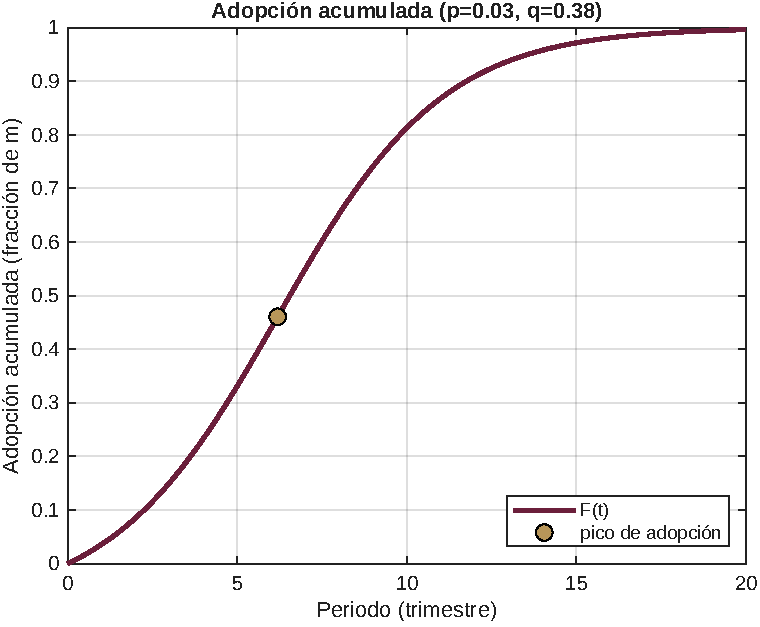
\includegraphics[width=\linewidth,height=0.58\textheight,keepaspectratio]{cap01_bass_acumulada.pdf}\\
  {\scriptsize Adopción acumulada $F(t)$}
  \column{0.48\textwidth}
  \centering
  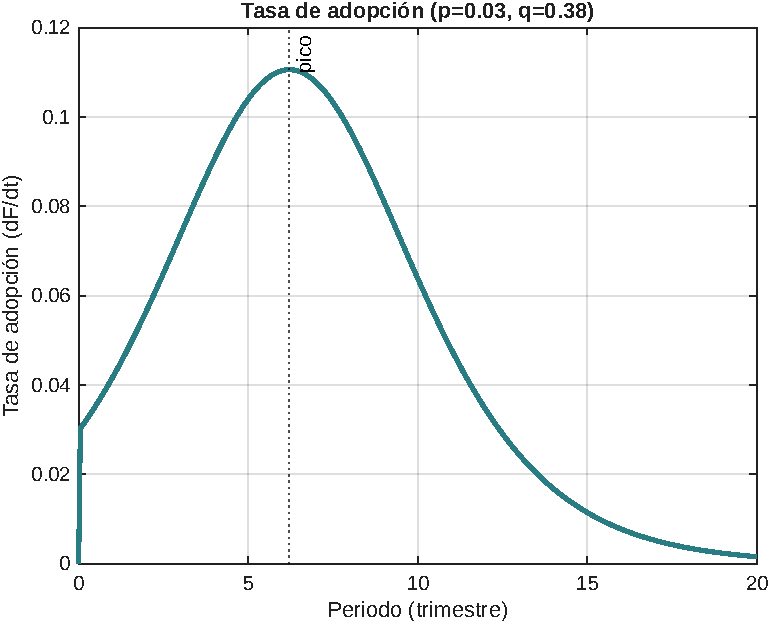
\includegraphics[width=\linewidth,height=0.58\textheight,keepaspectratio]{cap01_bass_tasa.pdf}\\
  {\scriptsize Tasa de adopción $dF/dt$}
\end{columns}
\vspace{4pt}
\begin{center}
  \small Pico en $t^\ast \approx 6.2$ periodos, con \textbf{46\,\%} del mercado ya adoptado en ese momento.
\end{center}
\fuente{elaboración propia, MATLAB, datos sintéticos.}
\end{frame}

\begin{frame}{Ejercicio propuesto: tres corridas}
\begin{columns}[T]
  \column{0.44\textwidth}
  \begin{exampleblock}{Casos (solo cambia $p$ y $q$)}
    \small
    \begin{itemize}
      \item[\textbf{A}] Innovación dominante:\\ $p=0.08$, $q=0.10$
      \item[\textbf{B}] Balance (por defecto):\\ $p=0.03$, $q=0.38$
      \item[\textbf{C}] Imitación dominante:\\ $p=0.01$, $q=0.55$
    \end{itemize}
  \end{exampleblock}
  \column{0.52\textwidth}
  \small
  \begin{tabular}{@{}lccc@{}}
    \toprule
    Caso & $t^\ast$ & \% en el pico & \% en $t=20$ \\
    \midrule
    A & \rule{1cm}{0.4pt} & \rule{1cm}{0.4pt} & \rule{1cm}{0.4pt} \\[4pt]
    B & \rule{1cm}{0.4pt} & \rule{1cm}{0.4pt} & \rule{1cm}{0.4pt} \\[4pt]
    C & \rule{1cm}{0.4pt} & \rule{1cm}{0.4pt} & \rule{1cm}{0.4pt} \\
    \bottomrule
  \end{tabular}
  \vspace{6pt}
  \begin{block}{Respondan con sus corridas}
    \scriptsize
    \begin{enumerate}
      \item ¿En qué caso el pico ocurre más tarde?
      \item ¿En qué caso la fase inicial es más plana?
      \item Propongan un canal digital real (app, red social, método de pago) y justifiquen a qué caso se parece.
    \end{enumerate}
  \end{block}
\end{columns}
\end{frame}

%------------------------------------------------
\section[Caso]{Estudio de caso}
%------------------------------------------------

\begin{frame}{Caso: la app de ahorro que \enquote{no despega}}
\begin{exampleblock}{Caso ficticio}
  Una fintech mexicana lanza una app de ahorro programado para trabajadores independientes. A los tres meses tiene \textbf{2{,}000} usuarios activos, frente a una proyección de \textbf{15{,}000}. La dirección discute: ¿el producto \enquote{no funciona} o necesita más tiempo?
\end{exampleblock}
\begin{columns}[T]
  \column{0.48\textwidth}
  \begin{block}{Lectura 1: innovación dominante}
    \small Crecimiento lento pero sostenido, sin señales de contagio entre usuarios.
  \end{block}
  \column{0.48\textwidth}
  \begin{block}{Lectura 2: imitación dominante}
    \small La app apenas sale del \enquote{valle} inicial; podría acelerar si el referido entre usuarios empieza a operar.
  \end{block}
\end{columns}
\end{frame}

\begin{frame}{Preguntas guía}
\begin{enumerate}
  \item ¿Qué evidencia adicional —más allá del conteo de usuarios activos— permitiría distinguir entre las dos lecturas?
  \vspace{3pt}
  \item Si el diagnóstico fuera \enquote{imitación en fase de valle}, ¿qué decisión de mercadotecnia sería la \textbf{más riesgosa} tomar ahora?
  \vspace{3pt}
  \item ¿Qué papel jugaría un \textbf{programa de referidos} en cambiar el balance entre $p$ y $q$?
  \vspace{3pt}
  \item ¿Qué tipo de evidencia usaría el equipo directivo para justificar su decisión ante la dirección general, y por qué debe ser de \textbf{fuente primaria}?
\end{enumerate}
\vspace{6pt}
\begin{alertblock}{Entregable}
  \small Solución escrita con las cuatro preguntas respondidas y una recomendación final justificada.
\end{alertblock}
\end{frame}

%------------------------------------------------
\section{Cierre}
%------------------------------------------------

\begin{frame}{Síntesis: tres ideas para llevarse}
\begin{block}{1. Curva vs.\ narrativa}
  \small La evolución del consumidor digital es una curva medible \emph{y} una narrativa editorial en versiones. Ambas son útiles; \textbf{solo una es evidencia}.
\end{block}
\begin{block}{2. Inteligente $\neq$ sostenible}
  \small Decisiones informadas por datos no son automáticamente de menor costo ambiental; la brecha actitud-conducta documenta esa distancia.
\end{block}
\begin{block}{3. Ventajas con evidencia desigual}
  \small Segmentación por comportamiento y reducción de fricción: bien sustentadas. Anticipación de tendencias: \textbf{la menos}.
\end{block}
\end{frame}

\begin{frame}{Autoevaluación rápida}
\footnotesize
\begin{enumerate}
  \item La serie \textit{Marketing X.0} debe entenderse principalmente como:
  \begin{itemize}
    \item[a)] un programa de investigación académica revisado por pares;
    \item[b)] \alt<2->{\textcolor{IPNguinda}{\textbf{una periodización editorial de consultoría alineada a la tecnología de cada momento}}}{una periodización editorial de consultoría alineada a la tecnología de cada momento};
    \item[c)] el primer marco teórico sobre comportamiento del consumidor digital.
  \end{itemize}
  \item En el modelo de Bass, si $q \gg p$, la curva de adopción muestra:
  \begin{itemize}
    \item[a)] crecimiento lineal y constante desde el inicio;
    \item[b)] \alt<2->{\textcolor{IPNguinda}{\textbf{una fase inicial plana seguida de adopción explosiva}}}{una fase inicial plana seguida de adopción explosiva};
    \item[c)] adopción inmediata de todo el mercado potencial.
  \end{itemize}
  \item La brecha actitud-conducta se refiere a:
  \begin{itemize}
    \item[a)] la diferencia de precio entre productos sostenibles y convencionales;
    \item[b)] \alt<2->{\textcolor{IPNguinda}{\textbf{la distancia entre la preferencia declarada y la compra real}}}{la distancia entre la preferencia declarada y la compra real};
    \item[c)] la brecha digital rural-urbana.
  \end{itemize}
\end{enumerate}
\end{frame}

\begin{frame}{Evidencias del portafolio}
\begin{block}{Pasos para subir los trabajos al portafolio}
    \begin{itemize}
    \item Accede a esta carpeta de evidencia: \url{https://drive.google.com/drive/folders/1sr_SAVkl_Mjil6ZRWz3O2mveMoZVW6cp?usp=sharing}
    \item Crea una carpeta con su nombre y organiza en dicha carpeta todos tus entregables en el semestre.
    \item Considera los tiempos limites establecidos para cada actividad.
    \end{itemize}
  \end{block}
\end{frame}

\begin{frame}{Evidencias del portafolio}
\small
\begin{columns}[T]
  \column{0.48\textwidth}
  \begin{block}{Exposición (8 min)}
    \scriptsize Narrativa de versiones vs.\ evolución verificable, con al menos un dato de INEGI o AMVO no citado en clase.
  \end{block}
  \begin{block}{Solución de casos}
    \scriptsize Caso de la fintech, cuatro preguntas y recomendación.
  \end{block}
  \column{0.48\textwidth}
  \begin{block}{Reporte de debate}
    \scriptsize \enquote{¿El consumo digital inteligente y el consumo sostenible son compatibles o están en tensión?} — al menos una postura apoyada en la brecha actitud-conducta.
  \end{block}
  \begin{block}{Reporte de práctica}
    \scriptsize Cuadro de los casos A, B y C del laboratorio, preguntas de comparación y canal digital real justificado.
  \end{block}
\end{columns}
\end{frame}

\begin{frame}{Para la próxima sesión (aprendizaje autónomo, 1 h)}
\begin{enumerate}
  \item Leer el comunicado más reciente de la \textbf{ENDUTIH} (INEGI) y extraer \textbf{tres cifras} no citadas en clase, con su fuente exacta.
  \vspace{4pt}
  \item Revisar la ficha editorial de \textit{Marketing 6.0} y anotar, en dos párrafos, si sus tendencias (inmersión, IA, IoT) ya son observables en algún servicio digital que usen a diario.
  \vspace{4pt}
  \item Ejecutar \texttt{cap01\_difusion\_bass\_\allowbreak interactivo.html} con los casos A, B y C y anotar el pico de adopción de cada uno.
\end{enumerate}
\end{frame}

\begin{frame}{Glosario de la sesión}
\small
\begin{description}
  \item[Brecha actitud-conducta] Distancia entre lo que un consumidor declara preferir y lo que efectivamente compra.
  \item[Consumo digital inteligente] Decisiones de compra informadas por datos y comparación en entornos digitales.
  \item[Coeficiente de innovación ($p$)] Propensión a adoptar de forma independiente. $p>0$; en clase, entre 0.01 y 0.08.
  \item[Coeficiente de imitación ($q$)] Cuánto depende la adopción del contagio social. $q\geq 0$; en clase, entre 0.10 y 0.55.
  \item[Mercado potencial ($m$)] Tamaño del mercado objetivo; normalizado a 1 (100\,\%).
  \item[\textit{Greenwashing}] Atributos ambientales comunicados que no se pueden verificar o que exageran su impacto real.
\end{description}
\end{frame}

\begin{frame}{Referencias}
\tiny
\begin{itemize}
  \item[] AMVO. (2026). \textit{Estudio de Venta Online 2026}. \url{https://amvo.org.mx/estudios}
  \item[] Bass, F. M. (1969). A new product growth for model consumer durables. \textit{Management Science, 15}(5), 215--227. \url{https://doi.org/10.1287/mnsc.15.5.215}
  \item[] INEGI. (2025). \textit{ENDUTIH 2024} (Comunicado de prensa 57/25). \url{https://www.inegi.org.mx/contenidos/saladeprensa/boletines/2025/endutih/ENDUTIH_24.pdf}
  \item[] INEGI. (2026). \textit{ENDUTIH 2025} (Comunicado de prensa 32/26). \url{https://www.inegi.org.mx/contenidos/saladeprensa/boletines/2026/endutih/ENDUTIH_25.pdf}
  \item[] Kotler, P., Kartajaya, H. y Setiawan, I. (2021). \textit{Marketing 5.0: Technology for humanity}. Wiley.
  \item[] Kotler, P., Kartajaya, H. y Setiawan, I. (2024). \textit{Marketing 6.0: The future is immersive}. Wiley.
  \item[] Organización de las Naciones Unidas. (2015). \textit{Objetivo 12: Garantizar modalidades de consumo y producción sostenibles}. \url{https://sdgs.un.org/goals/goal12}
  \item[] PROFECO. (2025). Entorno digital. \textit{Revista del Consumidor}, septiembre de 2025.
  \item[] Sheth, J. N. y Jain, V. (2026). \textit{Digital consumer behavior}. Routledge.
  \item[] Smith, W. R. (1956). Product differentiation and market segmentation as alternative marketing strategies. \textit{Journal of Marketing, 21}(1), 3--8. \url{https://doi.org/10.1177/002224295602100102}
  \item[] Solomon, M. R. (2017). \textit{Comportamiento del consumidor} (11.\textsuperscript{a} ed.). Pearson.
  \item[] Tversky, A. y Kahneman, D. (1974). Judgment under uncertainty: Heuristics and biases. \textit{Science, 185}(4157), 1124--1131. \url{https://doi.org/10.1126/science.185.4157.1124}
\end{itemize}
\end{frame}

\begin{frame}
    \begin{center}
        {\Large \textcolor{IPNguinda}{\textbf{Gracias}}}\\[6pt]
        {\color{IPNdorado}\rule{0.4\linewidth}{1.2pt}}\\[6pt]
        Dr. Aboud Barsekh-Onji \\
        \small Instituto Politécnico Nacional · ESCA Unidad Santo Tomás \\
        \small \texttt{ORCID: \href{https://orcid.org/0009-0004-5440-8092}{0009-0004-5440-8092}}
    \end{center}
\end{frame}

\end{document}
